\section{Durchführung}

\paragraph{a)}
\label{par:a}
Mithilfe eines Ringmodulators wird ein Amplitudenmoduliertes Signal erzeugt. Die dabei entstehende Schwebung wird anschließend mit einem
Oszilloskop visualisiert.

\paragraph{b)}
\label{par:b}
Es wird mit Hilfe eines Frequenzanalysators das Frequenzspektrum des in a) erzeugten Signals sichtbar gemacht.

\paragraph{c)}
\label{par:c}
Aufgabenteil a und b wird mit einer Diode zur Modulation wiederholt und die selben Signalseigenschaften untersucht.
Außerdem wird gezeigt das zusätzlich Oberwellen von $\omega_\text{T}$ auftreten.

\paragraph{d)}
\label{par:d}
Um das in amplitudenmodulierte Signal zu demodulieren wird ein Ringmodulator verwendet.
Mithilfe einer Schaltung gemäß Abbildung \ref{Abb14} und eines Multimeters wird die Proportionalität am Ausgang X mit dem Cosinus der Phase zwischen R und L gezeigt.

\begin{figure}
	\centering
	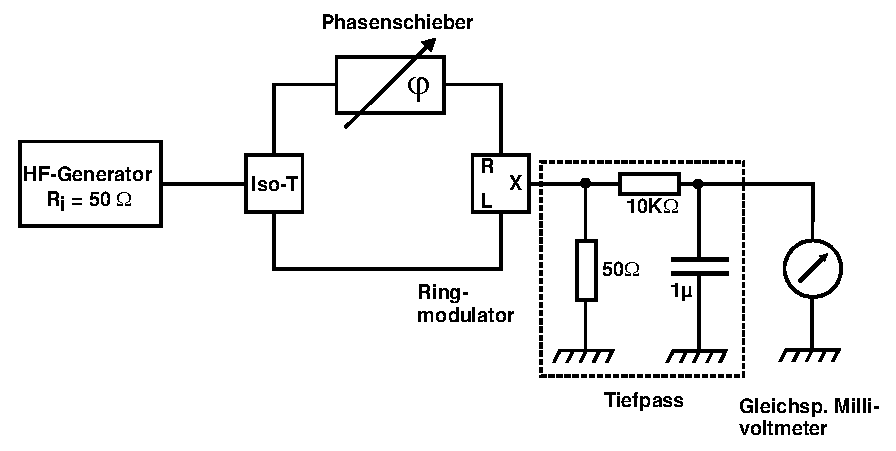
\includegraphics[width=\textwidth]{img/Abb14.pdf}
	\caption{Schaltung zum Aufnehmen der Beziehung zwischen Gleichspannung und Phase der Wechselspannung. \cite{FP}}
	\label{Abb14}
\end{figure}

\paragraph{e)}
\label{par:e}
Das Multimeter aus \ref{par:d} wird durch ein Oszilloskop ersetzt und das demodulierte Signal sichtbar gemacht.

\paragraph{f)}
\label{par:f}
Mit hilfe einer Gleichrichterdiode wird ein amplitudenmoduliertes Signal demoduliert.
Außerdem wird die Zeitabhängigkeit vor und hinter dem Tiefpass dargestellt.

\paragraph{g)}
\label{par:g}
Es wird ein frequenzmoduliertes Signal erzeugt, welches auf einem Oszilloskop dargestellt wird. Anschließend wird der Frequenzhub und
der Modulationsgrad ermittelt und das Frequenzspektrum untersucht.

\paragraph{h)}
\label{par:h}
Abschließend wird ein frequenzmoduliertes Signal demoduliert und das Ergebnis visualisiert.